% Options for packages loaded elsewhere
\PassOptionsToPackage{unicode}{hyperref}
\PassOptionsToPackage{hyphens}{url}
%
\documentclass[
]{book}
\usepackage{amsmath,amssymb}
\usepackage{lmodern}
\usepackage{iftex}
\ifPDFTeX
  \usepackage[T1]{fontenc}
  \usepackage[utf8]{inputenc}
  \usepackage{textcomp} % provide euro and other symbols
\else % if luatex or xetex
  \usepackage{unicode-math}
  \defaultfontfeatures{Scale=MatchLowercase}
  \defaultfontfeatures[\rmfamily]{Ligatures=TeX,Scale=1}
\fi
% Use upquote if available, for straight quotes in verbatim environments
\IfFileExists{upquote.sty}{\usepackage{upquote}}{}
\IfFileExists{microtype.sty}{% use microtype if available
  \usepackage[]{microtype}
  \UseMicrotypeSet[protrusion]{basicmath} % disable protrusion for tt fonts
}{}
\makeatletter
\@ifundefined{KOMAClassName}{% if non-KOMA class
  \IfFileExists{parskip.sty}{%
    \usepackage{parskip}
  }{% else
    \setlength{\parindent}{0pt}
    \setlength{\parskip}{6pt plus 2pt minus 1pt}}
}{% if KOMA class
  \KOMAoptions{parskip=half}}
\makeatother
\usepackage{xcolor}
\usepackage{color}
\usepackage{fancyvrb}
\newcommand{\VerbBar}{|}
\newcommand{\VERB}{\Verb[commandchars=\\\{\}]}
\DefineVerbatimEnvironment{Highlighting}{Verbatim}{commandchars=\\\{\}}
% Add ',fontsize=\small' for more characters per line
\usepackage{framed}
\definecolor{shadecolor}{RGB}{248,248,248}
\newenvironment{Shaded}{\begin{snugshade}}{\end{snugshade}}
\newcommand{\AlertTok}[1]{\textcolor[rgb]{0.94,0.16,0.16}{#1}}
\newcommand{\AnnotationTok}[1]{\textcolor[rgb]{0.56,0.35,0.01}{\textbf{\textit{#1}}}}
\newcommand{\AttributeTok}[1]{\textcolor[rgb]{0.77,0.63,0.00}{#1}}
\newcommand{\BaseNTok}[1]{\textcolor[rgb]{0.00,0.00,0.81}{#1}}
\newcommand{\BuiltInTok}[1]{#1}
\newcommand{\CharTok}[1]{\textcolor[rgb]{0.31,0.60,0.02}{#1}}
\newcommand{\CommentTok}[1]{\textcolor[rgb]{0.56,0.35,0.01}{\textit{#1}}}
\newcommand{\CommentVarTok}[1]{\textcolor[rgb]{0.56,0.35,0.01}{\textbf{\textit{#1}}}}
\newcommand{\ConstantTok}[1]{\textcolor[rgb]{0.00,0.00,0.00}{#1}}
\newcommand{\ControlFlowTok}[1]{\textcolor[rgb]{0.13,0.29,0.53}{\textbf{#1}}}
\newcommand{\DataTypeTok}[1]{\textcolor[rgb]{0.13,0.29,0.53}{#1}}
\newcommand{\DecValTok}[1]{\textcolor[rgb]{0.00,0.00,0.81}{#1}}
\newcommand{\DocumentationTok}[1]{\textcolor[rgb]{0.56,0.35,0.01}{\textbf{\textit{#1}}}}
\newcommand{\ErrorTok}[1]{\textcolor[rgb]{0.64,0.00,0.00}{\textbf{#1}}}
\newcommand{\ExtensionTok}[1]{#1}
\newcommand{\FloatTok}[1]{\textcolor[rgb]{0.00,0.00,0.81}{#1}}
\newcommand{\FunctionTok}[1]{\textcolor[rgb]{0.00,0.00,0.00}{#1}}
\newcommand{\ImportTok}[1]{#1}
\newcommand{\InformationTok}[1]{\textcolor[rgb]{0.56,0.35,0.01}{\textbf{\textit{#1}}}}
\newcommand{\KeywordTok}[1]{\textcolor[rgb]{0.13,0.29,0.53}{\textbf{#1}}}
\newcommand{\NormalTok}[1]{#1}
\newcommand{\OperatorTok}[1]{\textcolor[rgb]{0.81,0.36,0.00}{\textbf{#1}}}
\newcommand{\OtherTok}[1]{\textcolor[rgb]{0.56,0.35,0.01}{#1}}
\newcommand{\PreprocessorTok}[1]{\textcolor[rgb]{0.56,0.35,0.01}{\textit{#1}}}
\newcommand{\RegionMarkerTok}[1]{#1}
\newcommand{\SpecialCharTok}[1]{\textcolor[rgb]{0.00,0.00,0.00}{#1}}
\newcommand{\SpecialStringTok}[1]{\textcolor[rgb]{0.31,0.60,0.02}{#1}}
\newcommand{\StringTok}[1]{\textcolor[rgb]{0.31,0.60,0.02}{#1}}
\newcommand{\VariableTok}[1]{\textcolor[rgb]{0.00,0.00,0.00}{#1}}
\newcommand{\VerbatimStringTok}[1]{\textcolor[rgb]{0.31,0.60,0.02}{#1}}
\newcommand{\WarningTok}[1]{\textcolor[rgb]{0.56,0.35,0.01}{\textbf{\textit{#1}}}}
\usepackage{longtable,booktabs,array}
\usepackage{calc} % for calculating minipage widths
% Correct order of tables after \paragraph or \subparagraph
\usepackage{etoolbox}
\makeatletter
\patchcmd\longtable{\par}{\if@noskipsec\mbox{}\fi\par}{}{}
\makeatother
% Allow footnotes in longtable head/foot
\IfFileExists{footnotehyper.sty}{\usepackage{footnotehyper}}{\usepackage{footnote}}
\makesavenoteenv{longtable}
\usepackage{graphicx}
\makeatletter
\def\maxwidth{\ifdim\Gin@nat@width>\linewidth\linewidth\else\Gin@nat@width\fi}
\def\maxheight{\ifdim\Gin@nat@height>\textheight\textheight\else\Gin@nat@height\fi}
\makeatother
% Scale images if necessary, so that they will not overflow the page
% margins by default, and it is still possible to overwrite the defaults
% using explicit options in \includegraphics[width, height, ...]{}
\setkeys{Gin}{width=\maxwidth,height=\maxheight,keepaspectratio}
% Set default figure placement to htbp
\makeatletter
\def\fps@figure{htbp}
\makeatother
\setlength{\emergencystretch}{3em} % prevent overfull lines
\providecommand{\tightlist}{%
  \setlength{\itemsep}{0pt}\setlength{\parskip}{0pt}}
\setcounter{secnumdepth}{5}
\usepackage{booktabs}
\usepackage{amsthm}
\makeatletter
\def\thm@space@setup{%
  \thm@preskip=8pt plus 2pt minus 4pt
  \thm@postskip=\thm@preskip
}
\makeatother
\ifLuaTeX
  \usepackage{selnolig}  % disable illegal ligatures
\fi
\usepackage[]{natbib}
\bibliographystyle{apalike}
\IfFileExists{bookmark.sty}{\usepackage{bookmark}}{\usepackage{hyperref}}
\IfFileExists{xurl.sty}{\usepackage{xurl}}{} % add URL line breaks if available
\urlstyle{same} % disable monospaced font for URLs
\hypersetup{
  pdftitle={Using R to generate data for questions},
  pdfauthor={Craig Alexander \& Eilidh Jack},
  hidelinks,
  pdfcreator={LaTeX via pandoc}}

\title{Using R to generate data for questions}
\author{Craig Alexander \& Eilidh Jack}
\date{}

\begin{document}
\maketitle

{
\setcounter{tocdepth}{1}
\tableofcontents
}
\hypertarget{overview}{%
\chapter{Overview}\label{overview}}

In this session, we will take a look at how we can use R to generate data to create questions. The first example will work through question 1 of Paper 1 from the 2021 exam. You can access the \href{https://www.sqa.org.uk/sqa/files_ccc/NAH_Statistics_Paper1_2021.pdf}{paper} and \href{https://www.sqa.org.uk/sqa/files_ccc/mi_NAH_Statistics-Paper-1_mi_2021.pdf}{solutions} by clicking on the links. The second example will introduce how to generate data for a simple linear model.

\hypertarget{libraries}{%
\section{Libraries}\label{libraries}}

Throughout this tutorial, we will use some libraries within R. If you are logged into a University computer, please load the following libraries:

\begin{Shaded}
\begin{Highlighting}[]
\FunctionTok{library}\NormalTok{(tidyverse)}
\FunctionTok{library}\NormalTok{(truncnorm)}
\FunctionTok{library}\NormalTok{(gridExtra)}
\FunctionTok{library}\NormalTok{(BSDA)}
\FunctionTok{library}\NormalTok{(ggfortify)}
\end{Highlighting}
\end{Shaded}

If you would prefer to work through the examples on your own device, you will need to install the following libraries:

\begin{itemize}
\tightlist
\item
  \texttt{tidyverse}
\item
  \texttt{truncnorm}
\item
  \texttt{gridExtra}
\item
  \texttt{BSDA}
\item
  \texttt{ggfortify}
\end{itemize}

\hypertarget{paper-1-example}{%
\chapter{2021 Paper 1 Example}\label{paper-1-example}}

\hypertarget{question-1}{%
\section{Question 1}\label{question-1}}

In this example, we will take a look at question 1 from \href{https://www.sqa.org.uk/sqa/files_ccc/NAH_Statistics_Paper1_2021.pdf}{Paper 1} in 2021. This question is a report style question based on Google AI data of times taken to draw a cat or a dog. The example contains a stem and leaf diagram with the combined data and some summary statistics for both sets of drawings. Following this, a Mann-Whitney Test is carried out to test whether both samples have different average drawing times.

We will now look at how we can simulate a sample of the data from the question, by randomly sampling data for both groups using properties from their summary statistics

\hypertarget{generating-a-random-sample-of-data}{%
\subsection{Generating a random sample of data}\label{generating-a-random-sample-of-data}}

We can generate a random sample of data for both the categories using the summary statistics provided. As we can see from the stem and leaf diagram, the data have a lower bound, where we cannot observe any data below zero, as the data recorded are based on time elapsed.

In order to sample data of this form, we can use a variation of the Normal distribution called the \href{https://en.wikipedia.org/wiki/Truncated_normal_distribution}{truncated normal distribution}, which allows us to bound a Normal distribution through a given range.

To randomly sample data from this distribution, we can use the \texttt{rtruncnorm} function from the \texttt{truncnorm} package in R as follows:

\begin{Shaded}
\begin{Highlighting}[]
\NormalTok{sample\_cat }\OtherTok{\textless{}{-}} \FunctionTok{rtruncnorm}\NormalTok{(}\AttributeTok{n=}\DecValTok{121}\NormalTok{, }\AttributeTok{a=}\DecValTok{0}\NormalTok{, }\AttributeTok{b=}\DecValTok{14}\NormalTok{, }\AttributeTok{mean=}\FloatTok{5.4}\NormalTok{, }\AttributeTok{sd=}\FloatTok{2.31}\NormalTok{)}
\NormalTok{sample\_dog }\OtherTok{\textless{}{-}} \FunctionTok{rtruncnorm}\NormalTok{(}\AttributeTok{n=}\DecValTok{145}\NormalTok{, }\AttributeTok{a=}\DecValTok{0}\NormalTok{, }\AttributeTok{b=}\DecValTok{16}\NormalTok{, }\AttributeTok{mean=}\FloatTok{7.5}\NormalTok{, }\AttributeTok{sd=}\FloatTok{2.66}\NormalTok{)}
\end{Highlighting}
\end{Shaded}

The parameters required are defined as follows:

\begin{itemize}
\tightlist
\item
  \texttt{n} - the number of samples we wish to draw
\item
  \texttt{a} - the lower bound of the distribution (here, we will set this to 0)
\item
  \texttt{b} - the upper bound of the distribution (here, we have set this to be the ceiling of the max value for each group)
\item
  \texttt{mean} - the mean of each group
\item
  \texttt{sd} - the standard deviation of each group
\end{itemize}

Running the code above will produce a sample for both groups based on their relative summary statistics. We can check the summary statistics of our data using \texttt{summary()}

\begin{Shaded}
\begin{Highlighting}[]
\FunctionTok{summary}\NormalTok{(sample\_cat)}
\end{Highlighting}
\end{Shaded}

\begin{verbatim}
##    Min. 1st Qu.  Median    Mean 3rd Qu.    Max. 
##  0.3641  3.4919  4.7518  5.0838  6.3575 11.2882
\end{verbatim}

\begin{Shaded}
\begin{Highlighting}[]
\FunctionTok{summary}\NormalTok{(sample\_dog)}
\end{Highlighting}
\end{Shaded}

\begin{verbatim}
##    Min. 1st Qu.  Median    Mean 3rd Qu.    Max. 
##  0.2323  6.4623  8.1252  7.9339  9.3019 15.5964
\end{verbatim}

We can now compare these summary statistics to those of the real data provided in the paper and notice that our simulated data produces fairly similar summary statistics.

\textbf{Exercise}
Try editing some of the parameters in \texttt{rtruncnorm} to see how this changes the summary statistics you obtain.

\hypertarget{visualising-the-data}{%
\subsection{Visualising the data}\label{visualising-the-data}}

We can also check the distribution of our sampled data for comparison by visualising it using a histogram. The \texttt{ggplot2} library found in the \texttt{tidyverse} library provides several functions for data visualisation and has become more popular than base R graphics. We will use the \texttt{geom\_histogram()} function from the library in this example as follows:

\begin{Shaded}
\begin{Highlighting}[]
\NormalTok{dog\_hist }\OtherTok{\textless{}{-}} \FunctionTok{ggplot}\NormalTok{(}\FunctionTok{data.frame}\NormalTok{(sample\_dog),}\FunctionTok{aes}\NormalTok{(}\AttributeTok{x=}\NormalTok{sample\_dog))}\SpecialCharTok{+}
  \FunctionTok{geom\_histogram}\NormalTok{(}\AttributeTok{color=}\StringTok{"black"}\NormalTok{,}\AttributeTok{fill=}\StringTok{"white"}\NormalTok{) }\SpecialCharTok{+} 
            \FunctionTok{labs}\NormalTok{(}\AttributeTok{title=}\StringTok{"Average draw time of dogs"}\NormalTok{,}\AttributeTok{x=}\StringTok{"Time (s)"}\NormalTok{)}
\NormalTok{cat\_hist }\OtherTok{\textless{}{-}} \FunctionTok{ggplot}\NormalTok{(}\FunctionTok{data.frame}\NormalTok{(sample\_cat),}\FunctionTok{aes}\NormalTok{(}\AttributeTok{x=}\NormalTok{sample\_cat))}\SpecialCharTok{+}
  \FunctionTok{geom\_histogram}\NormalTok{(}\AttributeTok{color=}\StringTok{"black"}\NormalTok{,}\AttributeTok{fill=}\StringTok{"white"}\NormalTok{) }\SpecialCharTok{+} 
  \FunctionTok{labs}\NormalTok{(}\AttributeTok{title=}\StringTok{"Average draw time of cats"}\NormalTok{,}\AttributeTok{x=}\StringTok{"Time (s)"}\NormalTok{)}

\FunctionTok{grid.arrange}\NormalTok{(cat\_hist, dog\_hist,}\AttributeTok{ncol=}\DecValTok{2}\NormalTok{)}
\end{Highlighting}
\end{Shaded}

\begin{verbatim}
## `stat_bin()` using `bins = 30`. Pick better value with `binwidth`.
## `stat_bin()` using `bins = 30`. Pick better value with `binwidth`.
\end{verbatim}

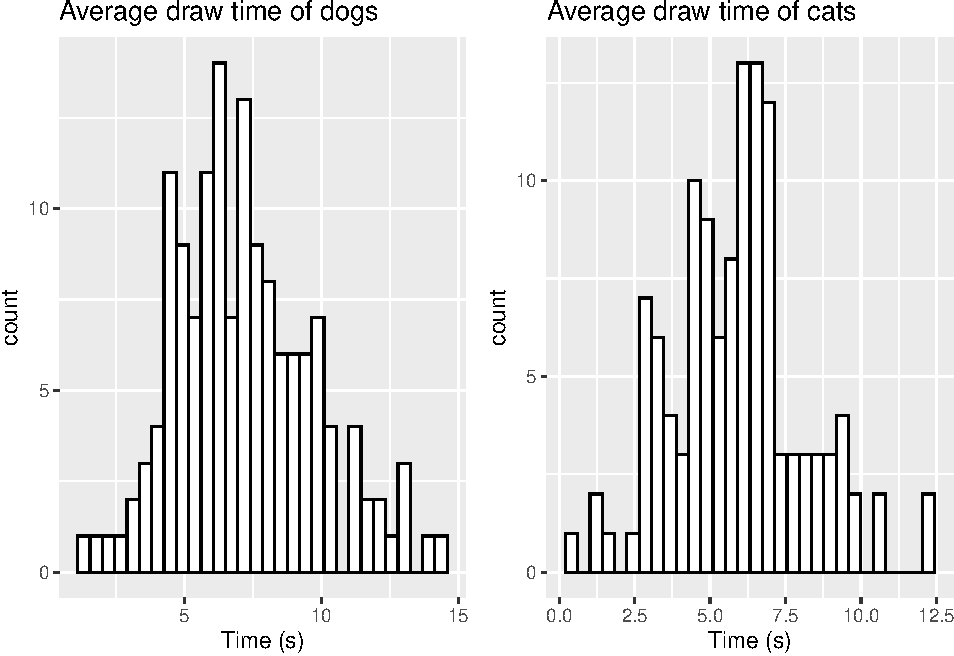
\includegraphics{bookdown-demo_files/figure-latex/histograms-1.pdf}

To create these histograms, the code above works in the following fashion:

\begin{itemize}
\tightlist
\item
  We first specify our data using \texttt{ggplot(data)}, where our data here is either group of samples.
\item
  To specify which variables we would like to select, we use the \texttt{aes()} argument. As we only have one sample of data in each case, we specify this using \texttt{x=data}.
\item
  We then generate the histogram using \texttt{geom\_histogram()}, where we can define the line colour using \texttt{color} and the filled colour of the bars using \texttt{fill}.
\item
  We can label our plot using the \texttt{labs} argument, where we can include a \texttt{title} and an \texttt{x} axis label
\end{itemize}

We can also alter the number of bins we use (\texttt{ggplot} will set a standard number of bins by default) using the \texttt{bins} argument. Let's alter the number of bins for the dog data to be 10

\begin{Shaded}
\begin{Highlighting}[]
\NormalTok{dog\_hist }\OtherTok{\textless{}{-}} \FunctionTok{ggplot}\NormalTok{(}\FunctionTok{data.frame}\NormalTok{(sample\_dog),}\FunctionTok{aes}\NormalTok{(}\AttributeTok{x=}\NormalTok{sample\_dog))}\SpecialCharTok{+}
  \FunctionTok{geom\_histogram}\NormalTok{(}\AttributeTok{color=}\StringTok{"black"}\NormalTok{,}\AttributeTok{fill=}\StringTok{"white"}\NormalTok{,}\AttributeTok{bins=}\DecValTok{10}\NormalTok{) }\SpecialCharTok{+} 
  \FunctionTok{labs}\NormalTok{(}\AttributeTok{title=}\StringTok{"Average draw time of dogs"}\NormalTok{,}\AttributeTok{x=}\StringTok{"Time (s)"}\NormalTok{)}
\end{Highlighting}
\end{Shaded}

\textbf{Exercise}
Try edit some of the inputs to the histogram plot. You can change the colour scheme, number of bins and the labels for the plot.

\hypertarget{setting-random-seeds-for-reproducibility}{%
\subsection{Setting random seeds for reproducibility}\label{setting-random-seeds-for-reproducibility}}

When we randomly sample data each time in R, we will obtain a different sample than before. Let's run our previous code twice to see if there is any differences:

\begin{Shaded}
\begin{Highlighting}[]
\NormalTok{sample\_dog1 }\OtherTok{\textless{}{-}} \FunctionTok{rtruncnorm}\NormalTok{(}\AttributeTok{n=}\DecValTok{145}\NormalTok{, }\AttributeTok{a=}\DecValTok{0}\NormalTok{, }\AttributeTok{b=}\DecValTok{16}\NormalTok{, }\AttributeTok{mean=}\FloatTok{7.5}\NormalTok{, }\AttributeTok{sd=}\FloatTok{2.66}\NormalTok{)}
\NormalTok{sample\_dog2 }\OtherTok{\textless{}{-}} \FunctionTok{rtruncnorm}\NormalTok{(}\AttributeTok{n=}\DecValTok{145}\NormalTok{, }\AttributeTok{a=}\DecValTok{0}\NormalTok{, }\AttributeTok{b=}\DecValTok{16}\NormalTok{, }\AttributeTok{mean=}\FloatTok{7.5}\NormalTok{, }\AttributeTok{sd=}\FloatTok{2.66}\NormalTok{)}

\FunctionTok{summary}\NormalTok{(sample\_dog1)}
\end{Highlighting}
\end{Shaded}

\begin{verbatim}
##    Min. 1st Qu.  Median    Mean 3rd Qu.    Max. 
##  0.4464  5.7736  7.3936  7.5150  9.2837 13.4899
\end{verbatim}

\begin{Shaded}
\begin{Highlighting}[]
\FunctionTok{summary}\NormalTok{(sample\_dog2)}
\end{Highlighting}
\end{Shaded}

\begin{verbatim}
##    Min. 1st Qu.  Median    Mean 3rd Qu.    Max. 
##  0.2391  5.3456  7.5616  7.4537  9.2504 13.4568
\end{verbatim}

We see that both samples produce different summary statistics. This can cause difficulty when you are working on a specific problem and want to design questions around the specific characteristics of the data you have sampled the first time.

We can force R to use the same random number generation by using the \texttt{set.seed()} function. Here, we specify the seed from the random number generator we want to use each time we generate samples. This number can be any number you wish to choose! The example below highlights how this works:

\begin{Shaded}
\begin{Highlighting}[]
\FunctionTok{set.seed}\NormalTok{(}\DecValTok{2023}\NormalTok{)}
\NormalTok{sample\_dog1 }\OtherTok{\textless{}{-}} \FunctionTok{rtruncnorm}\NormalTok{(}\AttributeTok{n=}\DecValTok{145}\NormalTok{, }\AttributeTok{a=}\DecValTok{0}\NormalTok{, }\AttributeTok{b=}\DecValTok{16}\NormalTok{, }\AttributeTok{mean=}\FloatTok{7.5}\NormalTok{, }\AttributeTok{sd=}\FloatTok{2.66}\NormalTok{)}
\FunctionTok{set.seed}\NormalTok{(}\DecValTok{2023}\NormalTok{)}
\NormalTok{sample\_dog2 }\OtherTok{\textless{}{-}} \FunctionTok{rtruncnorm}\NormalTok{(}\AttributeTok{n=}\DecValTok{145}\NormalTok{, }\AttributeTok{a=}\DecValTok{0}\NormalTok{, }\AttributeTok{b=}\DecValTok{16}\NormalTok{, }\AttributeTok{mean=}\FloatTok{7.5}\NormalTok{, }\AttributeTok{sd=}\FloatTok{2.66}\NormalTok{)}

\FunctionTok{summary}\NormalTok{(sample\_dog1)}
\end{Highlighting}
\end{Shaded}

\begin{verbatim}
##    Min. 1st Qu.  Median    Mean 3rd Qu.    Max. 
##   2.006   6.316   7.545   7.798   9.365  14.776
\end{verbatim}

\begin{Shaded}
\begin{Highlighting}[]
\FunctionTok{summary}\NormalTok{(sample\_dog2)}
\end{Highlighting}
\end{Shaded}

\begin{verbatim}
##    Min. 1st Qu.  Median    Mean 3rd Qu.    Max. 
##   2.006   6.316   7.545   7.798   9.365  14.776
\end{verbatim}

Here, we see we can produce the same data as the first sample by setting the seed prior to sampling.

\textbf{Exercise}
Try setting your own choice of random seed here and see how the summary statistics change.

\hypertarget{manually-editing-data}{%
\subsection{Manually editing data}\label{manually-editing-data}}

If we take a sample of data and perhaps wish to add some additional variables to mimic the original data closer, this can easily be done in R. Let's take a sample for the dog data but lower our boundary to 14 and visualise.

\begin{Shaded}
\begin{Highlighting}[]
\FunctionTok{set.seed}\NormalTok{(}\DecValTok{2023}\NormalTok{)}
\NormalTok{sample\_dog }\OtherTok{\textless{}{-}} \FunctionTok{rtruncnorm}\NormalTok{(}\AttributeTok{n=}\DecValTok{145}\NormalTok{, }\AttributeTok{a=}\DecValTok{0}\NormalTok{, }\AttributeTok{b=}\DecValTok{14}\NormalTok{, }\AttributeTok{mean=}\FloatTok{7.5}\NormalTok{, }\AttributeTok{sd=}\FloatTok{2.66}\NormalTok{)}

\FunctionTok{ggplot}\NormalTok{(}\FunctionTok{data.frame}\NormalTok{(sample\_dog),}\FunctionTok{aes}\NormalTok{(}\AttributeTok{x=}\NormalTok{sample\_dog)) }\SpecialCharTok{+}
  \FunctionTok{geom\_histogram}\NormalTok{(}\AttributeTok{color=}\StringTok{"black"}\NormalTok{,}\AttributeTok{fill=}\StringTok{"white"}\NormalTok{,}\AttributeTok{bins=}\DecValTok{12}\NormalTok{) }\SpecialCharTok{+} 
            \FunctionTok{labs}\NormalTok{(}\AttributeTok{title=}\StringTok{"Average draw time of dogs"}\NormalTok{,}\AttributeTok{x=}\StringTok{"Time(s)"}\NormalTok{)}
\end{Highlighting}
\end{Shaded}

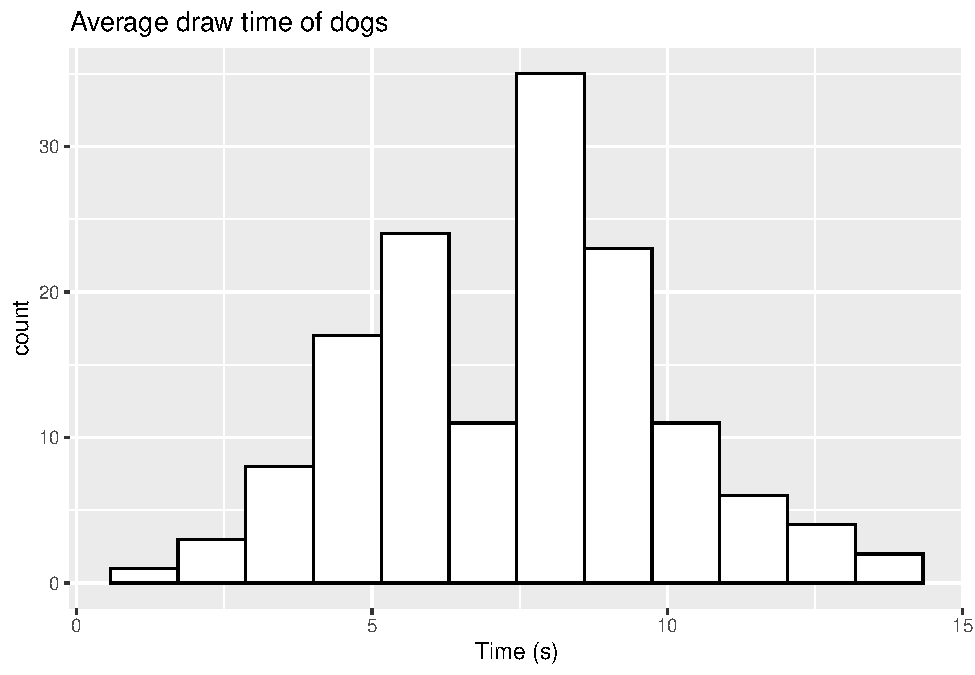
\includegraphics{bookdown-demo_files/figure-latex/lowsample-1.pdf}

When comparing this to the original data from the paper, we see that we do not observe the two outliers at 14.3 seconds and 15.2 seconds. In order to maintain the same sample size, we can reduce our samples here to be 143, and then manually add the two outliers. We can manually add these values as follows:

\begin{Shaded}
\begin{Highlighting}[]
\FunctionTok{set.seed}\NormalTok{(}\DecValTok{2023}\NormalTok{)}
\NormalTok{sample\_dog }\OtherTok{\textless{}{-}} \FunctionTok{rtruncnorm}\NormalTok{(}\AttributeTok{n=}\DecValTok{143}\NormalTok{, }\AttributeTok{a=}\DecValTok{0}\NormalTok{, }\AttributeTok{b=}\DecValTok{14}\NormalTok{, }\AttributeTok{mean=}\FloatTok{7.5}\NormalTok{, }\AttributeTok{sd=}\FloatTok{2.66}\NormalTok{)}
\NormalTok{sample\_dog }\OtherTok{\textless{}{-}} \FunctionTok{c}\NormalTok{(sample\_dog, }\FunctionTok{c}\NormalTok{(}\FloatTok{14.3}\NormalTok{,}\FloatTok{15.2}\NormalTok{))}

\FunctionTok{ggplot}\NormalTok{(}\FunctionTok{data.frame}\NormalTok{(sample\_dog),}\FunctionTok{aes}\NormalTok{(}\AttributeTok{x=}\NormalTok{sample\_dog)) }\SpecialCharTok{+}
  \FunctionTok{geom\_histogram}\NormalTok{(}\AttributeTok{color=}\StringTok{"black"}\NormalTok{,}\AttributeTok{fill=}\StringTok{"white"}\NormalTok{,}\AttributeTok{bins=}\DecValTok{12}\NormalTok{) }\SpecialCharTok{+} 
            \FunctionTok{labs}\NormalTok{(}\AttributeTok{title=}\StringTok{"Average draw time of dogs"}\NormalTok{,}\AttributeTok{x=}\StringTok{"Time (s)"}\NormalTok{)}
\end{Highlighting}
\end{Shaded}

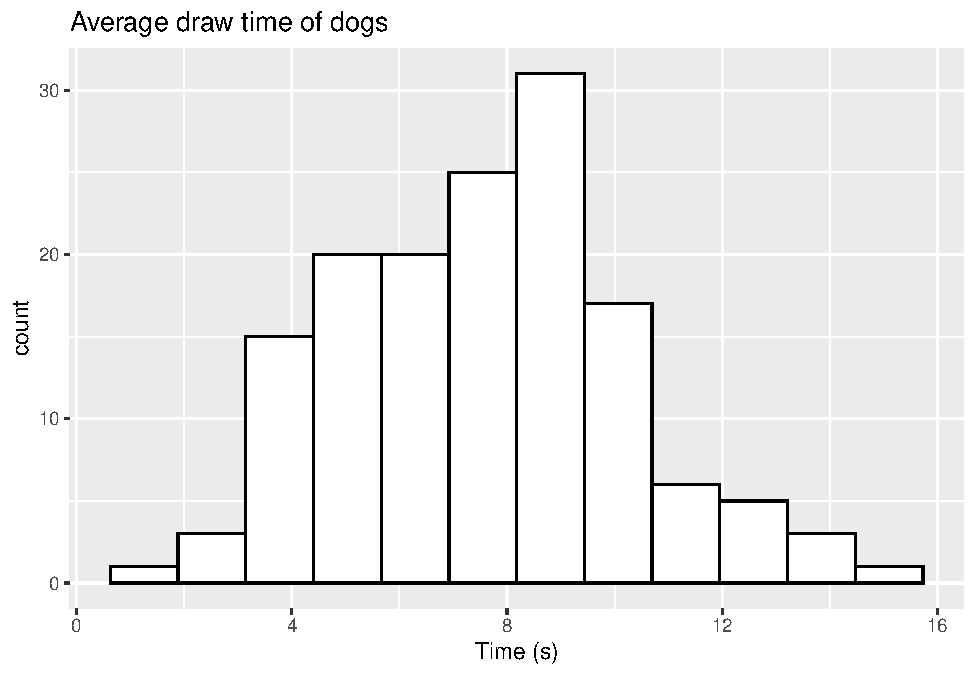
\includegraphics{bookdown-demo_files/figure-latex/modify-1.pdf}

We now observe the two additional values in the histogram. For a vector of data, we can easily add new values using the \texttt{c()} command. This can be done by specifying our original data first, and then including our additional variables in a new \texttt{c()} object. If we only wish to add one value, we do not need to use \texttt{c()}.

We can also make this update in a slightly different way. If we take our original sample of 145, we can directly replace two of the observations we have. We can replace the two highest values from our sampled data with the two outliers as follows:

\begin{Shaded}
\begin{Highlighting}[]
\FunctionTok{set.seed}\NormalTok{(}\DecValTok{2023}\NormalTok{)}
\NormalTok{sample\_dog }\OtherTok{\textless{}{-}} \FunctionTok{rtruncnorm}\NormalTok{(}\AttributeTok{n=}\DecValTok{145}\NormalTok{, }\AttributeTok{a=}\DecValTok{0}\NormalTok{, }\AttributeTok{b=}\DecValTok{14}\NormalTok{, }\AttributeTok{mean=}\FloatTok{7.5}\NormalTok{, }\AttributeTok{sd=}\FloatTok{2.66}\NormalTok{)}

\CommentTok{\# Order the data from higest to lowest}
\NormalTok{sample\_dog }\OtherTok{\textless{}{-}}\NormalTok{ sample\_dog[}\FunctionTok{order}\NormalTok{(sample\_dog,}\AttributeTok{decreasing=}\ConstantTok{TRUE}\NormalTok{)]}

\CommentTok{\# Replace the 2 highest values with our outliers}
\NormalTok{sample\_dog[}\DecValTok{1}\SpecialCharTok{:}\DecValTok{2}\NormalTok{] }\OtherTok{\textless{}{-}} \FunctionTok{c}\NormalTok{(}\FloatTok{14.3}\NormalTok{,}\FloatTok{15.2}\NormalTok{)}

\FunctionTok{ggplot}\NormalTok{(}\FunctionTok{data.frame}\NormalTok{(sample\_dog),}\FunctionTok{aes}\NormalTok{(}\AttributeTok{x=}\NormalTok{sample\_dog)) }\SpecialCharTok{+} \FunctionTok{geom\_histogram}\NormalTok{(}\AttributeTok{color=}\StringTok{"black"}\NormalTok{,}\AttributeTok{fill=}\StringTok{"white"}\NormalTok{,}\AttributeTok{bins=}\DecValTok{12}\NormalTok{) }\SpecialCharTok{+} 
            \FunctionTok{labs}\NormalTok{(}\AttributeTok{title=}\StringTok{"Average draw time of dogs"}\NormalTok{,}\AttributeTok{x=}\StringTok{"Time (s)"}\NormalTok{)}
\end{Highlighting}
\end{Shaded}

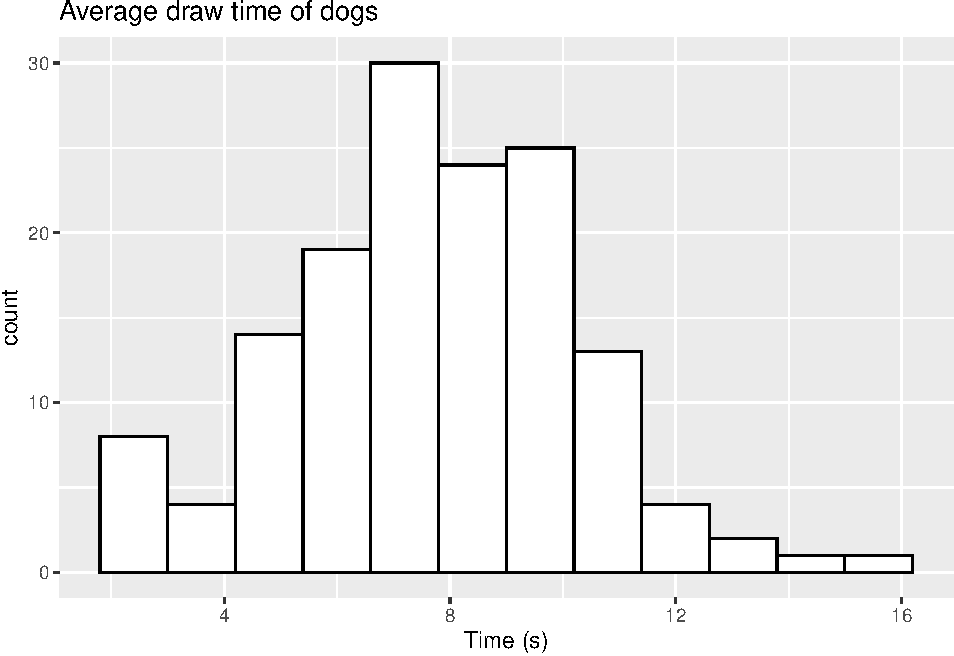
\includegraphics{bookdown-demo_files/figure-latex/lowsample2-1.pdf}
Here, we have used the \texttt{order} function to sort our data from the highest numerical observation to the lowest. The \texttt{decreasing=TRUE} argument sets this order from highest to lowest. If you wanted to replace the two lowest arguments, you can simply drop the \texttt{decreasing=TRUE} argument here. We then update the first two observations with our two outliers.

\textbf{Exercise}
Try replacing the two lowest values of your sampled data with the two identified outliers.

\hypertarget{sampling-from-different-distributions}{%
\subsection{Sampling from different distributions}\label{sampling-from-different-distributions}}

In this case, the data shown roughly takes the form of a Normal distribution. There are several cases where this may not be an appropriate distribution. R contains a full range of different distributions we can sample from. Some common choices are shown below:

\begin{itemize}
\tightlist
\item
  \texttt{rbinom()} - Sample from a Binomial distribution
\item
  \texttt{rchisq()} - Sample from a Chi-squared distribution
\item
  \texttt{rgamma()} - Sample from a Gamma distribution
\item
  \texttt{runif()} - Sample from a Uniform distribution
\item
  \texttt{rexp()} - Sample from an Exponential distribution
\end{itemize}

This list is not exhaustive, and R will contain libraries that will allow sampling from almost any known distribution.

\textbf{Exercise}
Carry out the steps we have worked through above, but this time using a different distribution of your choice. You can find information on what parameters need to be specified using the \texttt{?} notation before the function name (e.g.~\texttt{?rexp})

\hypertarget{performing-a-mann-whitney-test}{%
\subsection{Performing a Mann-Whitney Test}\label{performing-a-mann-whitney-test}}

We can carry out a Mann-Whitney test in R as follows

\begin{Shaded}
\begin{Highlighting}[]
\NormalTok{sample\_dog }\OtherTok{\textless{}{-}} \FunctionTok{rtruncnorm}\NormalTok{(}\AttributeTok{n=}\DecValTok{145}\NormalTok{, }\AttributeTok{a=}\DecValTok{0}\NormalTok{, }\AttributeTok{b=}\DecValTok{16}\NormalTok{, }\AttributeTok{mean=}\FloatTok{7.5}\NormalTok{, }\AttributeTok{sd=}\FloatTok{2.66}\NormalTok{)}
\NormalTok{sample\_cat }\OtherTok{\textless{}{-}} \FunctionTok{rtruncnorm}\NormalTok{(}\AttributeTok{n=}\DecValTok{121}\NormalTok{, }\AttributeTok{a=}\DecValTok{0}\NormalTok{, }\AttributeTok{b=}\DecValTok{14}\NormalTok{, }\AttributeTok{mean=}\FloatTok{5.4}\NormalTok{, }\AttributeTok{sd=}\FloatTok{2.31}\NormalTok{)}

\NormalTok{mann\_whitney }\OtherTok{\textless{}{-}} \FunctionTok{wilcox.test}\NormalTok{(sample\_dog,sample\_cat)}
\NormalTok{mann\_whitney}
\end{Highlighting}
\end{Shaded}

\begin{verbatim}
## 
##  Wilcoxon rank sum test with continuity correction
## 
## data:  sample_dog and sample_cat
## W = 13000, p-value = 1.33e-11
## alternative hypothesis: true location shift is not equal to 0
\end{verbatim}

The output from this test gives us the rank sum \texttt{W} and a p-value which can be used for question creation

\hypertarget{performing-a-z-test}{%
\section{Performing a z-test}\label{performing-a-z-test}}

We can perform a two-sample z test in R using the \texttt{z.test} function from the \texttt{BSDA} package. We can carry out this test as follows:

\begin{Shaded}
\begin{Highlighting}[]
\FunctionTok{z.test}\NormalTok{(sample\_cat,sample\_dog,}\AttributeTok{sigma.x=}\FloatTok{2.307}\NormalTok{,}\AttributeTok{sigma.y=}\FloatTok{2.655}\NormalTok{)}
\end{Highlighting}
\end{Shaded}

\begin{verbatim}
## 
##  Two-sample z-Test
## 
## data:  sample_cat and sample_dog
## z = -7.1488, p-value = 8.752e-13
## alternative hypothesis: true difference in means is not equal to 0
## 95 percent confidence interval:
##  -2.771824 -1.578983
## sample estimates:
## mean of x mean of y 
##  5.286729  7.462132
\end{verbatim}

Here, we specify the sample standard deviation for cats and dogs respectively. The output from the test gives us the z-statistic, p-value and 95\% confidence interval.

\hypertarget{linear-model-example}{%
\chapter{Linear model example}\label{linear-model-example}}

In this section we will introduce how to generate data for a linear model example using the linear model equation.

This example is based on the following question.

\hypertarget{question}{%
\section{Question}\label{question}}

A global ice cream company is interested in using linear regression to predict its ice cream waste (kg) based on the average temperatures of its store locations (\(^{\circ}\)C).

The estimated linear model is:

\[\hat{waste} = 597 - 10.91 \times temperature.\]

\begin{enumerate}
\def\labelenumi{\arabic{enumi}.}
\tightlist
\item
  What is the predicted waste for a store location whose average temperature is 18\(^{\circ}\)C? \emph{Provide your answer to two decimal places.}
\end{enumerate}

\begin{center}\rule{0.5\linewidth}{0.5pt}\end{center}

\begin{enumerate}
\def\labelenumi{\arabic{enumi}.}
\setcounter{enumi}{1}
\tightlist
\item
  The standard error for the slope coefficient is 0.92, which is associated with \(df=32\). Calculate a 95\% confidence interval for the slope parameter. \emph{Provide your answer to two decimal places.}
\end{enumerate}

Lower:\_\_\_\_\_\_
Upper:\_\_\_\_\_

\begin{enumerate}
\def\labelenumi{\arabic{enumi}.}
\setcounter{enumi}{2}
\tightlist
\item
  Suppose you performed a hypothesis test to test if average temperature is a significant predictor of ice cream waste. Working at a significance level of 5\%, would you expect the p-value of the hypothesis test to be:
\end{enumerate}

\begin{itemize}
\item
  \begin{enumerate}
  \def\labelenumi{(\Alph{enumi})}
  \tightlist
  \item
    greater than 0.05\\
  \end{enumerate}
\item
  \begin{enumerate}
  \def\labelenumi{(\Alph{enumi})}
  \setcounter{enumi}{1}
  \tightlist
  \item
    Cannot tell with the information provided\\
  \end{enumerate}
\item
  \begin{enumerate}
  \def\labelenumi{(\Alph{enumi})}
  \setcounter{enumi}{2}
  \tightlist
  \item
    less than 0.05
  \end{enumerate}
\end{itemize}

\hypertarget{generating-data}{%
\section{Generating data}\label{generating-data}}

In order to fit this linear model we need to generate two variables:

\begin{itemize}
\tightlist
\item
  Response variable (\(y\)): \(waste\) and
\item
  Explanatory variable (\(x\)): \(temperature\).
\end{itemize}

Crucially, these variables need to be associated with each other as shown in the linear model equation.

\hypertarget{explanatory-variable}{%
\subsection{Explanatory variable}\label{explanatory-variable}}

Let's start by generating our x-variable, \(temperature\). We will use a Normal distribution to do this since our variable is continuous.

\begin{Shaded}
\begin{Highlighting}[]
\NormalTok{temp}\OtherTok{\textless{}{-}}\FunctionTok{rnorm}\NormalTok{(}\AttributeTok{n=}\DecValTok{34}\NormalTok{, }\AttributeTok{mean=}\DecValTok{12}\NormalTok{, }\AttributeTok{sd=}\DecValTok{4}\NormalTok{)}
\end{Highlighting}
\end{Shaded}

The parameters required are defined as follows:

\begin{itemize}
\tightlist
\item
  \texttt{n} - the number of samples we wish to draw. In our question \(df=32\), so \(n=34\) (since for a simple linear model \(df=n-2\)).
\item
  \texttt{mean} - the mean temperature which our data will be centered on. Pick something sensible here, we have gone for \(12^{\circ}\)C.
\item
  \texttt{sd} - the standard deviation for \(temperature\). Again go for something that seems sensible (high enough to show some variability, but not too high that the values at the extreme are no longer sensible). This can take a bit of trial and error.
\end{itemize}

Let's take a look at our simulated data to check that is looks sensible. To do this we will the \texttt{geom\_histogram()} function that we used in our previous example.

\begin{Shaded}
\begin{Highlighting}[]
\FunctionTok{ggplot}\NormalTok{(}\FunctionTok{data.frame}\NormalTok{(temp),}\FunctionTok{aes}\NormalTok{(}\AttributeTok{x=}\NormalTok{temp)) }\SpecialCharTok{+} 
  \FunctionTok{geom\_histogram}\NormalTok{(}\AttributeTok{color=}\StringTok{"black"}\NormalTok{,}\AttributeTok{fill=}\StringTok{"white"}\NormalTok{, }\AttributeTok{bins=}\DecValTok{10}\NormalTok{) }\SpecialCharTok{+} 
            \FunctionTok{labs}\NormalTok{(}\AttributeTok{x=}\StringTok{"Average temperature"}\NormalTok{)}
\end{Highlighting}
\end{Shaded}

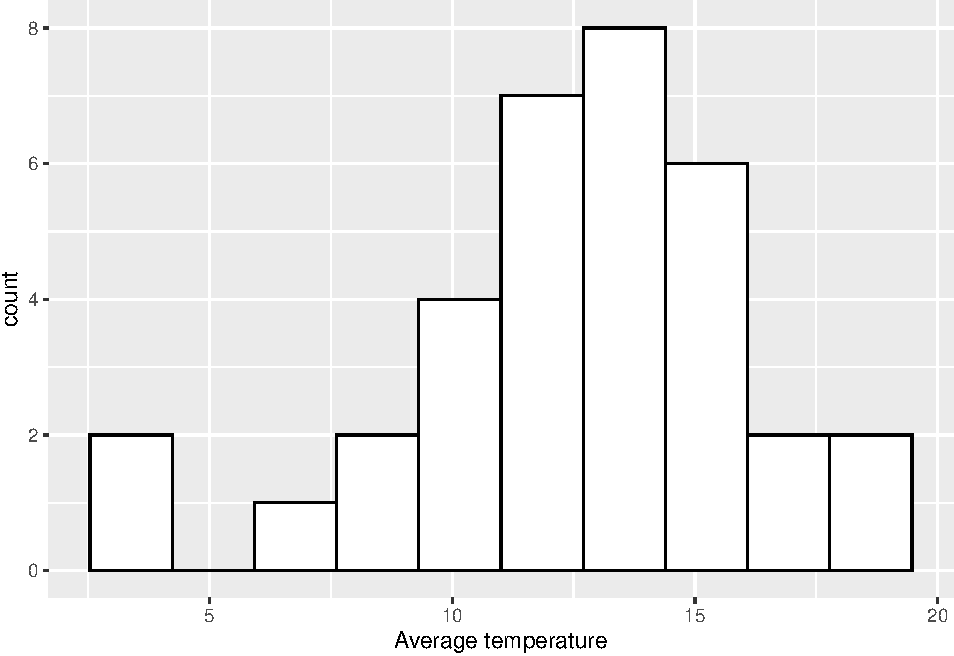
\includegraphics{bookdown-demo_files/figure-latex/xhist-1.pdf}

\textbf{Exercise}
Change the values of the \texttt{mean} and \texttt{sd} in the code above and plot a histogram of the newly simulated \(x\) value to see how the data changes.

\hypertarget{using-a-linear-model-to-generate-the-response}{%
\subsection{Using a linear model to generate the response}\label{using-a-linear-model-to-generate-the-response}}

In order to generate the response variable \(y\) we need to choose a sensible linear model which will relate the explantory variable \(x\) to the response variable \(y\).

To specify a simple linear model we need to choose two values, the intercept, \(\alpha\), and the slope, \(\beta\). In this example we want to estimate ice cream waste from average temperature, we are therefore going to assume there is a \emph{negative} relationship between these variables, i.e.~the warmer it is, the more ice cream you will sell! Therefore, the slope parameter (\(\beta\)) should be negative. The size of this will depend on what you think is a sensible interpretation. Here let's go for -10.65, so for every unit increase in average temperature, ice cream waste decreases by 10.65kg. For the intercept, again think about a sensible value based on the context. Remember this value is where the regression line will cut the y-axis. Let's choose 591. The choice for \(\alpha\) and \(\beta\) will be subjective, and might take some trial and error before deciding on your final values. Just make sure that the interpretation of the final model is sensible.

We can now generate the response variable, \(y\) as follows:

\begin{Shaded}
\begin{Highlighting}[]
\NormalTok{waste}\OtherTok{\textless{}{-}}\DecValTok{591} \SpecialCharTok{{-}} \FloatTok{10.65}\SpecialCharTok{*}\NormalTok{temp}
\end{Highlighting}
\end{Shaded}

where

\begin{itemize}
\tightlist
\item
  591 is our chosen value for \(\alpha\),
\item
  -10.65 is our chosen value for \(\beta\),
\item
  \texttt{temp} is the x-variable we have already simulated.
\end{itemize}

Let's now produce a scatterplot of our data using \texttt{ggplot2}. We will use a similar structure to the plots we have produced previously but we will use the \texttt{geom\_point()} function to produce a scatterplot as follows:

\begin{Shaded}
\begin{Highlighting}[]
\NormalTok{data}\OtherTok{\textless{}{-}}\FunctionTok{data.frame}\NormalTok{(}\AttributeTok{waste=}\NormalTok{waste, }\AttributeTok{temp=}\NormalTok{temp)}

\FunctionTok{ggplot}\NormalTok{(data, }\FunctionTok{aes}\NormalTok{(}\AttributeTok{x=}\NormalTok{temp, }\AttributeTok{y=}\NormalTok{waste)) }\SpecialCharTok{+} 
  \FunctionTok{geom\_point}\NormalTok{() }\SpecialCharTok{+} 
  \FunctionTok{labs}\NormalTok{(}\AttributeTok{x=}\StringTok{"Average temperature"}\NormalTok{, }\AttributeTok{y=}\StringTok{"Ice cream waste"}\NormalTok{)}
\end{Highlighting}
\end{Shaded}

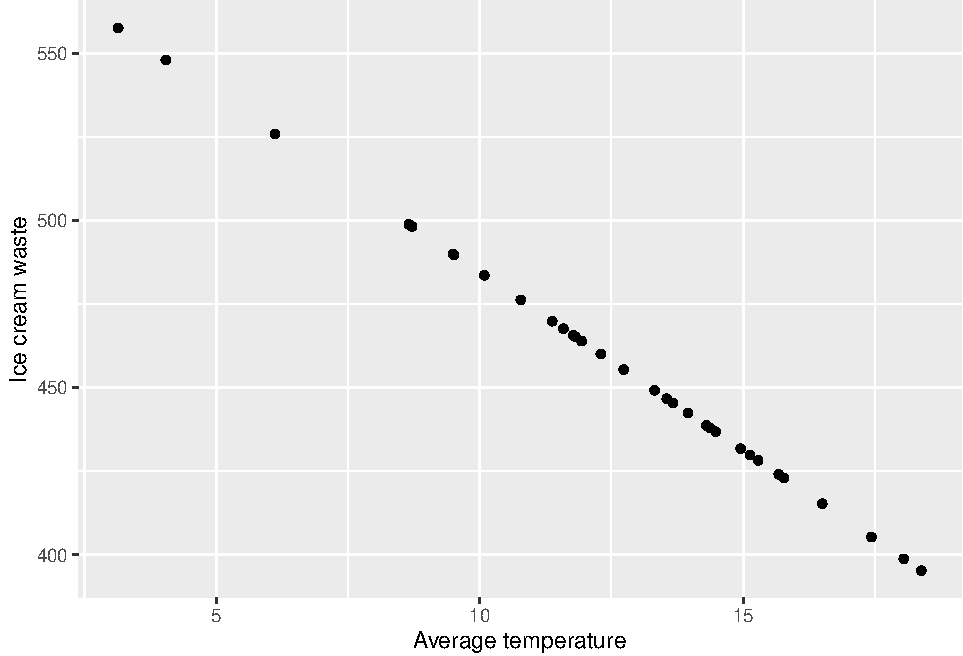
\includegraphics{bookdown-demo_files/figure-latex/xyscatter-1.pdf}

To create this scatterplot we first had to store our two variables in a \emph{dataframe} which we called \texttt{data}. Here we are creating a dataframe with two columns which we have given the same names as the two data vectors we have already created, namely \texttt{waste} and \texttt{temp}. In these columns we are simply storing the data vectors we have simulated above. We then create the scatterplot which works as follows:

\begin{itemize}
\tightlist
\item
  First we specify our data using \texttt{ggplot(data)}.
\item
  We then specify the variables we want to plot using the \texttt{aes()} argument, where \texttt{x=temp} and \texttt{y=waste}.
\item
  We then generate the scatterplot using \texttt{geom\_point()}. Here we have used the default values so we don't need to specify anything within this function.
\item
  Finally, we label our x and y axis using the \texttt{labs} function.
\end{itemize}

Now, you may have noticed that our scatterplot has identified an issue with the data we have generated. The code we have used has produced a perfect linear relationship between \(temperature\) and \(waste\). This does not seem realistic so we need to add some random noise to \(y\). We can do this by adding some randomly generated values from a normal distribution with mean 0. Think of this as adding residuals to our model.

\begin{Shaded}
\begin{Highlighting}[]
\NormalTok{waste}\OtherTok{\textless{}{-}}\DecValTok{591} \SpecialCharTok{{-}} \FloatTok{10.65}\SpecialCharTok{*}\NormalTok{temp }\SpecialCharTok{+} \FunctionTok{rnorm}\NormalTok{(}\AttributeTok{n=}\DecValTok{34}\NormalTok{, }\AttributeTok{mean=}\DecValTok{0}\NormalTok{, }\AttributeTok{sd=}\DecValTok{20}\NormalTok{)}
\end{Highlighting}
\end{Shaded}

We always want the model residuals to be centered on 0, so the mean within \texttt{rnorm()} should be 0. The level of variability within \(y\) can be controlled via the standard deviation (\texttt{sd}). Again, this might take some trial and error to get something you are happy with.

Let's take a look at the scatterplot with our newly generated response.

\begin{Shaded}
\begin{Highlighting}[]
\NormalTok{data}\OtherTok{\textless{}{-}}\FunctionTok{data.frame}\NormalTok{(}\AttributeTok{waste=}\NormalTok{waste, }\AttributeTok{temp=}\NormalTok{temp)}

\FunctionTok{ggplot}\NormalTok{(data, }\FunctionTok{aes}\NormalTok{(}\AttributeTok{x=}\NormalTok{temp, }\AttributeTok{y=}\NormalTok{waste)) }\SpecialCharTok{+} 
  \FunctionTok{geom\_point}\NormalTok{() }\SpecialCharTok{+} 
  \FunctionTok{labs}\NormalTok{(}\AttributeTok{x=}\StringTok{"Average temperature"}\NormalTok{, }\AttributeTok{y=}\StringTok{"Ice cream waste"}\NormalTok{)}
\end{Highlighting}
\end{Shaded}

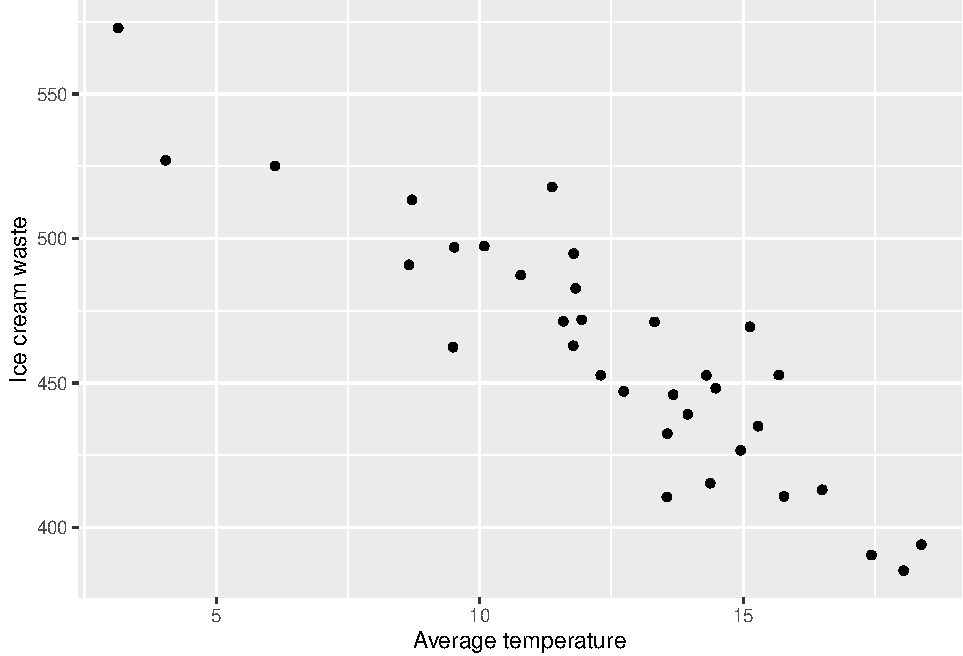
\includegraphics{bookdown-demo_files/figure-latex/xyscatter2-1.pdf}

That looks better!

\textbf{Exercise}
1. Change the values of \(\alpha\) and \(\beta\) in the code above to see how the relationship between \(x\) and \(y\) changes.
2. Alter the value of \texttt{sd} in the code above to control the level of variation in the \(y\).

\hypertarget{fitting-a-linear-model}{%
\section{Fitting a linear model}\label{fitting-a-linear-model}}

Now that we have simulated values for \(temperature\) and \(waste\) we can now fit a linear model and generate output that can be used to create questions.

\begin{Shaded}
\begin{Highlighting}[]
\NormalTok{model}\OtherTok{\textless{}{-}}\FunctionTok{lm}\NormalTok{(waste}\SpecialCharTok{\textasciitilde{}}\NormalTok{temp)}
\FunctionTok{summary}\NormalTok{(model)}
\end{Highlighting}
\end{Shaded}

\begin{verbatim}
## 
## Call:
## lm(formula = waste ~ temp)
## 
## Residuals:
##     Min      1Q  Median      3Q     Max 
## -38.514 -11.412  -2.084  10.421  45.052 
## 
## Coefficients:
##             Estimate Std. Error t value Pr(>|t|)    
## (Intercept) 596.9391    11.8702   50.29  < 2e-16 ***
## temp        -10.9101     0.9153  -11.92 2.62e-13 ***
## ---
## Signif. codes:  0 '***' 0.001 '**' 0.01 '*' 0.05 '.' 0.1 ' ' 1
## 
## Residual standard error: 18.85 on 32 degrees of freedom
## Multiple R-squared:  0.8162, Adjusted R-squared:  0.8104 
## F-statistic: 142.1 on 1 and 32 DF,  p-value: 2.62e-13
\end{verbatim}

Note that the estimates for \(\alpha\) and \(\beta\) are slightly different to the values we used to generate the data. This is because of the random noise we added when generating our response variable. The values are fairly similar though. Notice how these values correspond with the linear model used in the question at the top on the page, and how we have used the standard error from the output table when asking for a 95\% CI for the slope parameter (although this may be beyond the scope for the AH stats cirriculum).

\hypertarget{adding-the-linear-model-line-to-a-scatterplot}{%
\section{Adding the linear model line to a scatterplot}\label{adding-the-linear-model-line-to-a-scatterplot}}

We can now add our fitted model and 95\% confidence interval to the scatterplot of our data using the following code.

\begin{Shaded}
\begin{Highlighting}[]
\FunctionTok{ggplot}\NormalTok{(data, }\FunctionTok{aes}\NormalTok{(}\AttributeTok{x=}\NormalTok{temp, }\AttributeTok{y=}\NormalTok{waste)) }\SpecialCharTok{+} 
  \FunctionTok{geom\_point}\NormalTok{() }\SpecialCharTok{+} 
  \FunctionTok{labs}\NormalTok{(}\AttributeTok{x=}\StringTok{"Average temperature"}\NormalTok{, }\AttributeTok{y=}\StringTok{"Ice cream waste"}\NormalTok{)}\SpecialCharTok{+}
  \FunctionTok{geom\_smooth}\NormalTok{(}\AttributeTok{method=}\StringTok{"lm"}\NormalTok{, }\AttributeTok{se=}\ConstantTok{TRUE}\NormalTok{)}
\end{Highlighting}
\end{Shaded}

\begin{verbatim}
## `geom_smooth()` using formula 'y ~ x'
\end{verbatim}

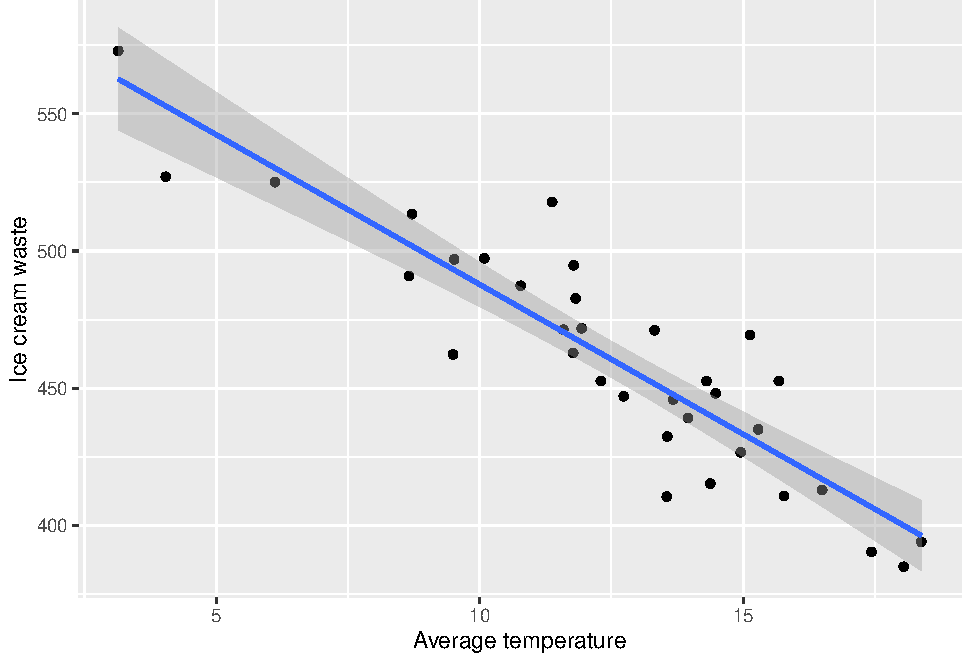
\includegraphics{bookdown-demo_files/figure-latex/xyscatter3-1.pdf}

To generate this plot we have used the same code as previously and added the \texttt{geom\_smooth()} with the following arguments:

\begin{itemize}
\tightlist
\item
  \texttt{method\ =\ lm} - fit a linear model line to the plot.
\item
  \texttt{se\ =\ TRUE} - display a confidence interval around the line. This can be removed by setting \texttt{se=FALSE}.
\end{itemize}

\hypertarget{producing-model-diagnostics}{%
\section{Producing model diagnostics}\label{producing-model-diagnostics}}

We can use the \texttt{autoplot()} function in the \texttt{ggfortify} library to create diagnostic plots for our linear model using \texttt{ggplot2} as follows:

\begin{Shaded}
\begin{Highlighting}[]
\FunctionTok{autoplot}\NormalTok{(model)}
\end{Highlighting}
\end{Shaded}

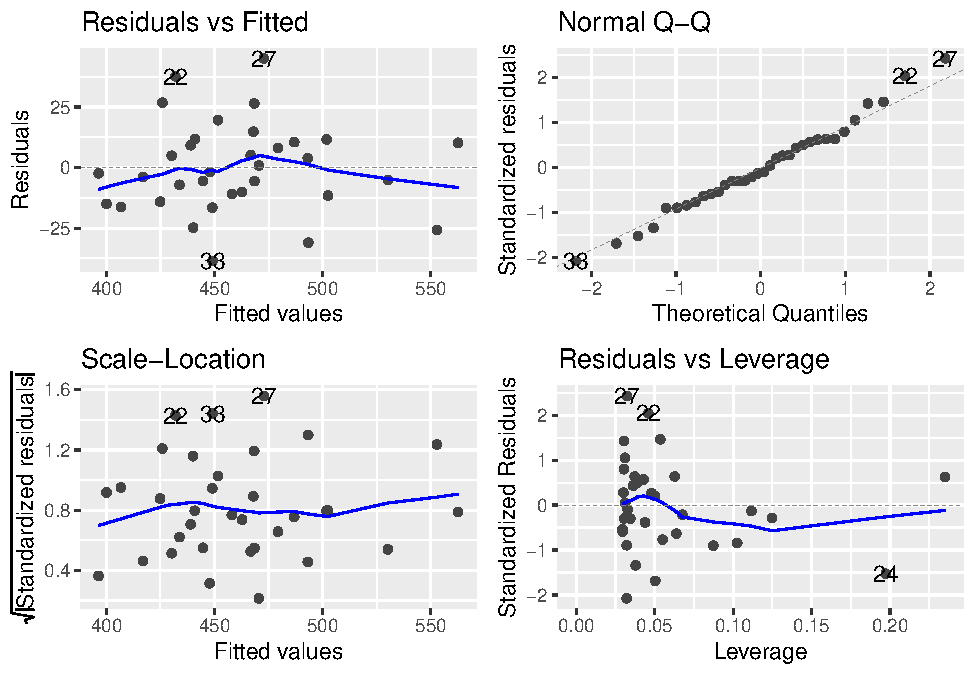
\includegraphics{bookdown-demo_files/figure-latex/modeldiag-1.pdf}

\hypertarget{calculating-quantities-of-interest}{%
\section{Calculating quantities of interest}\label{calculating-quantities-of-interest}}

You can also calculate quantities such as \(S_{xx}, S_{yy}\) and \(S_{xy}\) to be used in questions for calcuating estimates by hand.

\begin{Shaded}
\begin{Highlighting}[]
\NormalTok{S.xx }\OtherTok{\textless{}{-}} \FunctionTok{sum}\NormalTok{((temp }\SpecialCharTok{{-}} \FunctionTok{mean}\NormalTok{(temp))}\SpecialCharTok{\^{}}\DecValTok{2}\NormalTok{)}
\NormalTok{S.yy }\OtherTok{\textless{}{-}} \FunctionTok{sum}\NormalTok{((waste }\SpecialCharTok{{-}} \FunctionTok{mean}\NormalTok{(waste))}\SpecialCharTok{\^{}}\DecValTok{2}\NormalTok{)}
\NormalTok{S.xy }\OtherTok{\textless{}{-}} \FunctionTok{sum}\NormalTok{((temp }\SpecialCharTok{{-}} \FunctionTok{mean}\NormalTok{(temp)) }\SpecialCharTok{*}\NormalTok{ (waste }\SpecialCharTok{{-}} \FunctionTok{mean}\NormalTok{(waste)))}

\NormalTok{r }\OtherTok{\textless{}{-}}\NormalTok{ S.xy}\SpecialCharTok{/}\NormalTok{(}\FunctionTok{sqrt}\NormalTok{(S.xx}\SpecialCharTok{*}\NormalTok{S.yy))}
\NormalTok{beta }\OtherTok{\textless{}{-}}\NormalTok{ S.xy}\SpecialCharTok{/}\NormalTok{S.xx}
\NormalTok{alpha }\OtherTok{\textless{}{-}} \FunctionTok{mean}\NormalTok{(waste) }\SpecialCharTok{{-}}\NormalTok{ beta}\SpecialCharTok{*}\FunctionTok{mean}\NormalTok{(temp)}

\NormalTok{r}
\end{Highlighting}
\end{Shaded}

\begin{verbatim}
## [1] -0.9034156
\end{verbatim}

\begin{Shaded}
\begin{Highlighting}[]
\NormalTok{beta}
\end{Highlighting}
\end{Shaded}

\begin{verbatim}
## [1] -10.91007
\end{verbatim}

\begin{Shaded}
\begin{Highlighting}[]
\NormalTok{alpha}
\end{Highlighting}
\end{Shaded}

\begin{verbatim}
## [1] 596.9391
\end{verbatim}

\hypertarget{summary}{%
\section{Summary}\label{summary}}

Using \texttt{R} to generate data can be a quick and simple way to create practice questions for students. It can also be helpful to demonstrate certain properties when introducing concepts in class. Another benefit is to allow the creation of multiple variants of the same question, all with slighty different data, and therefore slightly different answers. This can be particularly helpful for revision questions that students can attempt more than once, or in assessments so that all students have slightly different questions/answers.

However, in general we would advise using real data when introducing/demonstrating concepts in class as this allows students to appreciate the use of statistics in real-life scenarios and also allows for discussions around dealing with messy data.

  \bibliography{book.bib,packages.bib}

\end{document}
